\documentclass[tikz,border=5mm]{standalone}
\usepackage{amsmath}

\begin{document}
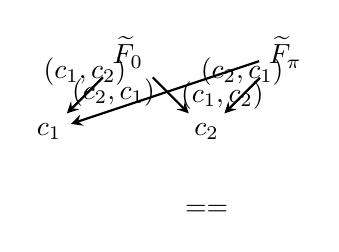
\begin{tikzpicture}[node distance=2cm]
    % Define styles for nodes
    \tikzset{
        mynode/.style={circle, draw, fill=blue!30, text width=4em, align=center},
        arrow/.style={->, thick, >=stealth}
    }

    % Nodes representing the functions and variables
    \node (F0) at (0,0) {$\widetilde{F}_0$};
    \node (Fpi) at (2,0) {$\widetilde{F}_\pi$};
    \node (c1) at (-1,-1) {$c_1$};
    \node (c2) at (1,-1) {$c_2$};

    % Arrows representing the arguments and equality
    \draw[arrow] (F0) -- node[above]{$(c_1, c_2)$} (c1);
    \draw[arrow] (F0) -- node[right]{$(c_1, c_2)$} (c2);
    \draw[arrow] (Fpi) -- node[above]{$(c_2, c_1)$} (c2);
    \draw[arrow] (Fpi) -- node[left]{$(c_2, c_1)$} (c1);

    % Equality symbol
    \node (eq) at (1,-2) {=$=$};
\end{tikzpicture}
\end{document}